\documentclass[a4paper,12pt]{article}
\usepackage[utf8]{inputenc}
\usepackage[T1]{fontenc}
\usepackage{algpseudocode}
\usepackage{algorithm}
\usepackage[magyar]{babel}
\usepackage{indentfirst}
\usepackage{biblatex}
\bibliography{intro}
\usepackage{amsmath}
\usepackage{graphicx}
\usepackage{url}
\frenchspacing
\author{Belényesi Roland}

\begin{document}
\section{Bevezetés}
A nagy adat (big data) napjainkban az egyik vezető cím az informatikai terminológiák körében, különböző címekkel ellátva, mint: 
\textsl{Sikerhez és boldogsághoz vezet a big data}~\cite{ori} vagy 
\textsl{Új korszak kezdődött a tudományban és}~\cite{oria}. Olyannyira megnőtt a kereslet a nagy adattal foglalkozó szakemberek iránt, hogy már az informatikán kívül is megjelent, Hal Varian, a híres közgazdász --aki egyben Google vezető közgazdásza-- szerint a \textsl{következő 10 éven belül az egyik legvonzóbb szakma lesz az adatokkal foglalkozó állás}. ~\cite{varian}. De mit is jelent pontosan? Nincs explicit meghatározás a fogalomra, de Doug Laney 2001-es definíciója egy jó kindulópontnak tekinthető: az adatok nagy mennyiségben (volume), gyorsan (velocity) és különböző formátumban (variety) jelennek meg (3V's)~\cite{3v}. Azonban, ma már kiegészíthetjük ezt a fogalmat még 4V-vel: bizonyosság (veracity) és érték (value), adategyezés (variability) és megjelenítés (visualization).~\cite{7v} Az adatmennyiség amit előállítunk exponenciálisan növekszik olyan szintre, aminek tárolását, menedzselését és elemzését már nem tudjuk megoldani a saját, lokális erőforrásainkon belül az eddig megszokott adatelemzési eszközökkel, mint például Microsoft Excel, vagy különböző relációs adatbázis technológiák által.
Becslések~\cite{2020} szerint az adatok mennyisége kétévente duplázódik, így 2020-ra az összekézben forgó adatmennyiség elérheti a 44 zetabájtnyi (vagy 44 trillió gigabájtnyi) mennyiséget.
\linebreak

A ,,big data'' lehetőséget biztosít arra, hogy ezeket az adatokat ne csak tároljuk, hanem új módokon tanuljunk belőle, értéket állítsunk elő, többet megtudjunk ügyfeleinkről, a saját üzleti folyamatainkról, ami versenyelőnyhöz vezethet. E mellett az áttörő kutatások számát is megnövelheti azáltal, hogy rejtett összefüggéseket mutat meg.~\cite{brk} 

A cloud computing, és új technológiák megszületése és az, hogy a fizikai világ egyre jobban átterelődik az online térbe, új nehézségeket állít elő mind az adatokat kiszolgáló, mind az adatokat elemző infrastruktúrák számára. Ezek a problémák komoly gondot jelentek az informatikai iparnak, mivel érintik az fizikai manifesztációt (hardver), mind az ezt vezérlő és feldolgozó réteget (szoftver és algoritmus). Ezek a problémák,~\cite{dst} --amelyek a tradícionális adattárház technológiákra jellemzőek-- többek között származhatnak a hiba-tolerancia hiányából, a sokféle adatfajtából, a párhuzamosság hiányából, mely azt eredményezi, hogy a mai technológia fejlettség (és a központi számítási egységek fizikailag limitáltsága miatt) nem lesz megfelelő számítási teljesítmény a megnövekedett adatmennyiség menedzselésére.

\section{A dolgozat célja}
q
A technológia fejlődése és a számítási teljesítmény megnövekedése hozta létre azt az üzleti igényt~\cite{rta}, hogy egyre gyorsabban, egyre nagyobb adatmennyiség feldolgozása történjen meg. Ilyen igény például:csalás felderítés~\cite{fraud}, "dolgok" internete (IoT)~\cite{iot} vagy alkalmazás monitoring~\cite{ganalitycs}. Ez az adatfeldolgozási sebesség olyan szintre eljutott, hogy közel valós időben, az adat keletkezése után megtörténhet ennek feldolgozása. Ilyen gyorsaságú adatfeldolgozásra csak elosztott rendszerek segítségével vagyunk képesek,~\cite{ucl} amelyek felépítésükből fakadóan sok lehetőség és költség jellemez, amelyeket a későbbiekben fogok kifejteni. A dolgozatomban használt Apache Flink (mely az Apache Foundation egyik legújabb és legmodernebb terméke) platform közel 40 millió elem feldolgozására képes egy 40 magos architektúrán másodpercenként.~\cite{flink}.  \linebreak

Ahhoz, hogy ezt az adatmennyiséget ki tudjuk elemezni és ajánlásokat tudjunk adni, gépi tanulásra van szükségünk. A gépi tanulás az informatikának és a matematikának egy olyan ága, amely az adatok folyamatos betáplálása során új ismereteket szolgáltat, megpróbál előrejelzéseket adni anélkül, hogy explicit módon be lenne erre programozva. ~\cite{ml}. A gépi tanulás egy olyan fajtáját fogom alkalmazni, ahol a termékek és felhasználóktól szerzett adatokból a lehető legpontosabban próbáljuk megjósolni, hogy milyen termék szerepelhet a felhasználó preferencialistája elején. Célom, hogy elosztott módon felépítsem az algoritmust, megnézzem, hogy milyen esetekben érdemes a párhuzamosítás, hol van az a határ, ahol a felépítésből fakadó többletköltség és komplexitás ellenére is megéri párhuzamos architektúrát alkalmazni. 
\linebreak

A választott metódus a sztochasztikus gradiens leszállás (SGD, stochastic gradient descent)~\cite{sgd}, amely egy olyan egyszerűsítési illetve optimalizációs eljárás, ahol adott célfüggvény gradiensét folyamatosan, iteratív módon számoljuk ki. Dolgozatomban megtervezem Apache Flinkben az SGD algoritmust, összehasonlítom a teljesítményét a már implementált algoritmusokkal és megkezdem a szükséges módosítások implementálást.

\section{Elosztottság}
A megnövekedett fizikai modellezési és katonai problémák miatt már 1950-es évektől kezdve felmerült az a kérdés, hogy hogyan lehetne összetett számítási feladatokat minél gyorsabban, egyszerűbben elvégezni. ~\cite{cocke} Rájöttek, hogy a problémákat olyan részproblémákra kell bontani, melyek megoldása egymástól független, így párhuzamosan is megoldhatóak, így jött létre a párhuzamos programozás. \linebreak
Párhuzamos programozás következő lépéseként jött létre az elosztott rendszerekre való igény, mely esetében a számolások már nem csak az adott számítási egységben különülnek el, hanem jóval több, akár különböző fizikai lokáción levő számítógép is ugyanannak a problémának egy számítását végzi. Azonban az ily módon elért számítási teljesítmény növekedés a komplexitás megnövekedésével is jár. Ezt a komplexitást különböző keretrendszerek elfedik, így biztosítva a lehetőséget elosztott alapon működő alkalmazások fejlesztésére. A komplexitás növekedése mellett a lehetőségeink is korlátozottak egy elosztott rendszer esetén. \linebreak \linebreak

Egy elosztott fájlrendszer esetén a fájljaink blokkokra vannak osztva a klaszter különböző csomópontjai (node) között.Ezek a különböző fájlblokkok másolatai elérhetőek különböző (logikai és/vagy fizika) lokációkon, mellyel biztosítjuk, hogy hardver meghibásodás esetén is elérhető legyen az adat. E mellett a rendszerben lévő névcsomópont (namenode) tárolja a fájlok és a hozzátartozó blokkok helyét. ~\cite{hdfs}
--TODO bővíteni

\subsection{Hibatűrés}

Az informatikai rendszerek összetettségének növekedésével megnő annak a valószínűsége, hogy a rendszerünk (vagy az alkalmazásunk) nem fogja a tőle elvárt, korrekt és pontos kimenetet biztosítani. Ezek a hibafaktorok lehetnek hardver (tároló lemez kiesés) vagy szoftver (rossz adat partícionálás) esetleg a köztes szoftverből (middleware) származóak. Ahhoz, hogy megbízható rendszert építsünk, lényeges, hogy a tervezett rendszer a különböző komponensek hibáját (közel) maximálisan tudja kijavítani. Az elosztott rendszerek kliens-szerver architektúra szerinte vannak felépítve, ahol távoli eljáráshívásoknál (RPC) kommunikálunk. Különböző mechanizmusokkal kell garantálnunk a hívás megérkezését, a hibák kijavítását és korrigálását. Ezek a különböző mechanizmusok lehetnek ~\cite{szemantika	}:

\begin{itemize}
\item Kliens nem találja a szervert, ezért a szervernek tájékoztatnia kell a klienst a kimaradásról
\item Kliens és szerver is megfelelően működik, viszont hálózati hiba miatt a hívás nem jut el a szerverig, esetleg a szerver válasza nem jut el a klienshez. Ilyen esetekben időkorlát (timeout) bevezetése egy jó megoldás, ami során újra küldjük a hívást
\item Hívásoknak idempotensnek kell lennie, tehát a többszöri azonos hívás futtatás sem fog hibát okozni a rendszerben
\end{itemize}

Amikor a szerver összeomlik olyanfajta szemantikákat kell alkalmaznunk, amely biztosítja a klienst a szerver állapotáról, illetve a szerver felépülés esetén tájékoztatja a klienst a jelenlegi állapotáról. \linebreak
Különböző hibatűrési szinteket vállalhatunk a hibatűrö rendszerünkkel: ~\cite{akka}

\begin{itemize}
\item Nincs semmilyen garancia az üzenet megérkezésére
\item At-most once (legfeljebb egyszer): Minden üzenet legfeljebb egyszer kézbesítésre kerül, de ezeknek az üzeneteknek egy rész nem jut el a címzetthez (üzenetek elveszhetnek).
\item At-least once (legalább egyszer): Minden üzenet legalább egyszer kézbesítésre kerül, de az üzenetek többször is eljuthatnak egy címzetthez, ami duplikált rekordokhoz vezethez (de semmiképpen nem veszik el)
\item Exactly once (Pontosan egyszer): Minden üzenet pontosan egyszer kerül kézbesítésre és fogadásra, nincs elveszett és duplikált üzenet sem.
\item Garantáljuk az üzenet elküldését pontosan egyszer, és ezek az üzenetek helyes sorrendben érkeznek meg.
\end{itemize}

Nem minden alkalmazás/szolgáltatás szegmensnek van szüksége arra, hogy mindig maximális pontosságú kimenetet adjon, ez az ún. részleges hiba tolerancia. 
--TODO bővíteni
-exactly once, at most once, etc

\subsection{Google fájl rendszer}
Google 2003-ban megalkotta a google fájl rendszert (GFS, Google File System)~\cite{gfs}, ami napjaink elosztott, hibatűrö rendszereinek az alapja. Tervezésénél fontos szempont volt, hogy skálázható, megbízható, elérhető és magas teljesítménnyel rendelkező legyen mindezt úgy, hogy adat-intenzív applikációk alapját fogja szolgálni. Figyelembe vették, hogy a komponens (mind adat, mind hardver oldalon) hibák inkább általánosak, mint kivételek, így az architektúra tervezésénél ez különös figyelmet kapott. E mellett relatív nagy fájlokra szabták (~64 megabájt) és fájlok felülírása helyett (overwrite) 
hozzáfűzték (append) az adatokat a létező fájlokhoz. Az elrendezés könyvtár alapú, a fájlokat névtér és fájl név alapján lehet azonosítani. Támogatja a megszokott létrehozás, törlés, megnyitás, olvasás és írás operátorokat, de bevezet kettő újat is a legoptimálisabb működés miatt: pillanatkép (snapshot) aminek segítségével a fájlrendszer pillanatnyi állapotról lehet mentést készíteni és párhuzamos hozzáfűzés (record append) ami lehetővé teszi, hogy egyszerre több kliens is tudjon egy fájlt írni. 

\begin{figure}[ht!]
\centering
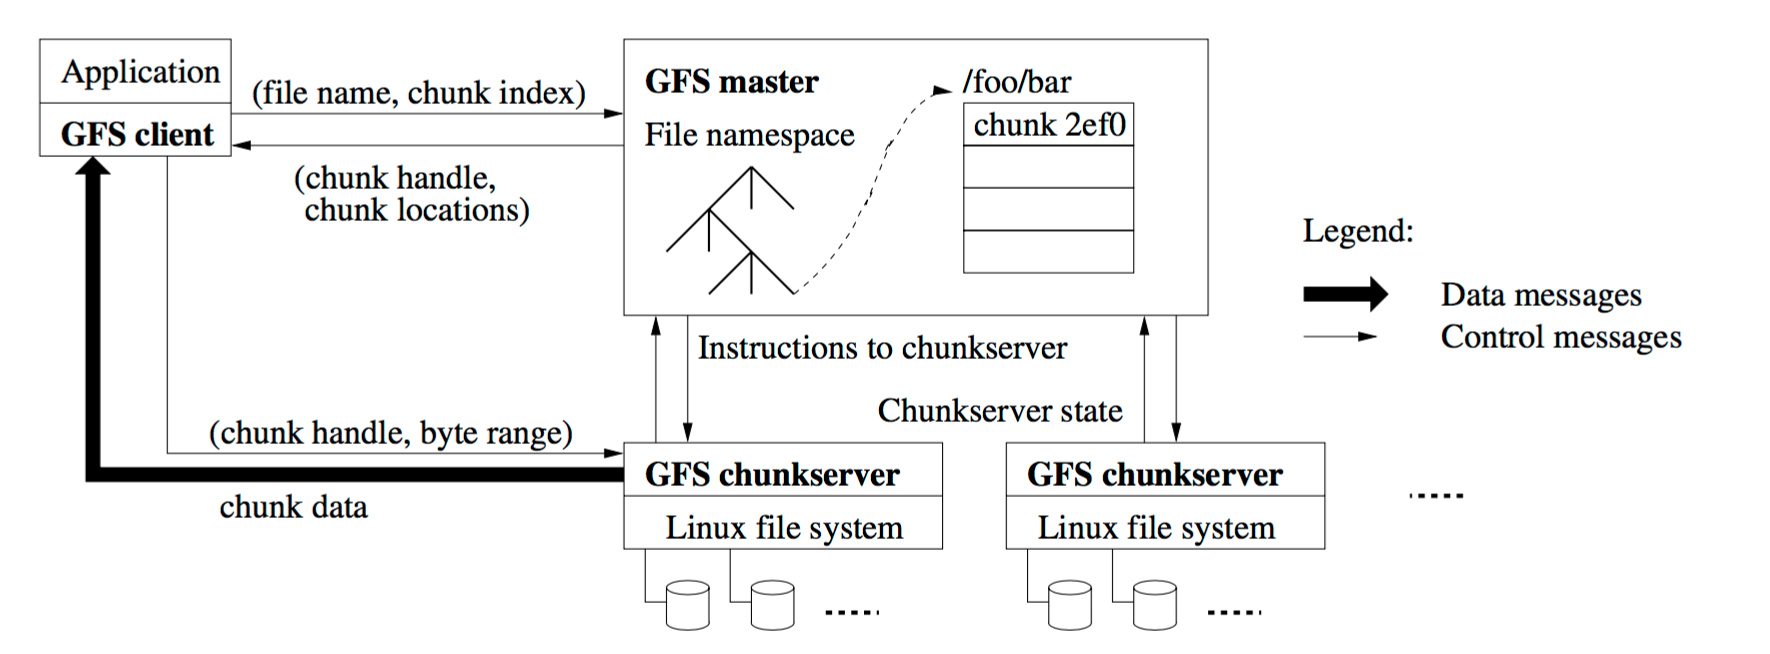
\includegraphics[width=130mm, height=100mm, keepaspectratio]{img/gfs.png}
\caption{Google fájl rendszer felépítése \label{gfs}}
\end{figure}

A fájlokat 64 megabájtos részekre (chunk) osztják, amit egy 64 kilobájtos fájl (chunk handle) kezel. Különböző szerverek (chunk server) tárolják a részeket, és minden fájlból három másolat készül a nagyobb konzisztencia érdekében. Az állapotkezelést és utasításokat mester-szolga (master-slave) módon építették fel, mester tárolja memóriában a metaadatokat (névtér, fájl helyek és fájl - > chunk leképzést). Ezen kívül biztosítva van az automatikusan, pár másodperc alatt feléledő a rendszer, kritikus, infrastruktúra hiba esetén.

\subsection{CAP tétel}
Az elosztott rendszerek tervezésekor és használatakor három képessséget várunk el elsősorban: legyen konzisztens (consistency), elérhető (availability) és partícionálás-tűrő (partition tolerance). 
\begin{itemize}
\item Konzisztencia: Bármelyik csomópontból kérdezem le az adatokat, mindig helyes választ kapok. Elosztott rendszereknél a konzisztencia megtartásához elengedhetetlen, hogy a csomópontok kommunikáljanak egymással. 
\item Elérhető: Bármelyik időpillanatban kapok választ egy kérés küldése után
\item Partícionálás-tűrő: Ha --a teljes hálózati kieséstől eltekintve-- egy csomópont eltűnik a hálózatról, akkor is kapok választ a rendszertől.
\end{itemize}
A CAP tétel kimondja ~\cite{cap}, hogy ebből a háromból legfeljebb kettő lehet igaz egy adott időpillanatban. Azonban a valóság nem ennyire letisztult, különböző rendszerek különböző prioritással veszik figyelembe a három alapképességet, így korlátozottan megtalálhatjuk a három alapképességet egy modern elosztott rendszerben. ~\cite{ecap}

\subsection{Párhuzamos kötegelt adatfeldolgozás}
A kétezres évek elején és közepén, a megfelelő számítási kapacitás hiányában a párhuzamos adatfeldolgozás általában \textsl{kötegelt} (batch) módon történt. Felhasználói interakció nélkül, megadott időközönként történik a nagy mennyiségű adat feldolgozása. Előnye, hogy akkor futhat a program, amikor a rendszer leterheltsége alacsony, ezzel biztosítva az egyenletes kihasználtságot. Mivel a parancsok automatikusan futnak le, ezért kisebb az üres, nem számítással töltött idő.~\cite{batch}.

\subsection{MapReduce}
A Google által fejlesztett MapReduce volt az első olyan szélesebb körben is elismert programozási modell, ami lehetővé tette, hogy nagymennyiségű adatot is lehessen feldolgozni párhuzamosan, elosztott módon. ~\cite{mapreduce} Az adatokat <kulcs, érték> párokra bontjuk, ahol a kulcs egy referencia, ami hivatkozik az adatra, míg az érték maga az adat. A bemenet az adat, míg a kimenet a köztes <kulcs, érték> pár. Ezt az ún. Map függvény valósítja meg, amit a felhasználónak kell biztosítania. A köztes <kulcs, érték> párt a felhasználó által írt Reduce függvény dolgozza fel. A Reduce függvényben a köztes <kulcs, érték> párok összegzése  zajlik, tehát megkeressük a vizsgált kulcshoz az összes értéket. \linebreak
Az egyik klasszikus példa a szószámolás, ahol meg kell számolnunk azt, hogy a bemeneti adatunk szavai milyen mennyiséggel fordulnak elő.

(forrás:http://kickstarthadoop.blogspot.hu/2011/04/word-count-hadoop-map-reduce-example.html)
\begin{figure}[ht!]
\centering
\includegraphics[width=80mm]{img/wordcountflow.jpg}
\caption{MapReduce alkalmazása  szószámoló példán keresztül. \label{wordcountflow}}
\end{figure}

Elsőként a bemeneti adatunkat (szövegfájl), sorokra bontjuk, majd a sorokat szavakra és a hozzájuk tartozó előfordulási értékekre (Map). Az így előállt <kulcs, érték> párokat aggregálom, majd összefésülöm (Reduce). A végső kimenet pedig ezeknek a összesített pároknak az összessége.

A ma használt keretrendszerek, az egyszerű ötletnek és magas absztrakciós szintnek köszönhetően lehetővé teszik, hogy a felhasználónak csak a konkrét adatfeldolgozó kóddal kelljen dolgoznia, mivel a keretrendszer elfedi az elosztott számítási komplexitást. ~\cite{hadoop}


\subsection{Adatfolyam alapú feldolgozás}
Mit is tekinthetünk adatfolyamnak? Olyan adatfeldolgozó motort, mely arra van tervezve, hogy végtelen és rendezetlen adatsorokat dolgozzon fel. Eddig az ilyen rendszereket alapvetően alacsony pontossággal és/vagy megbízhatatlansággal vádolták, mely csak spekulálni tud az egyes adatok valódi értékéről. Elmondhatjuk, hogy jobb megértést tud biztosítani a problémán az, hogy ha a végtelen adatunkat valós időben dolgozzuk fel, mivel az esetek többségében az adatunk elavul, csak egy limitált időkorláton belül tudjuk értelmezni, illetve hasznos információkat kinyerni. 
Lambda architektúra a maga idejében egy rendkívül jó megoldás volt, biztosítva az alacsony válaszidő és a pontosság egyvelegét. Ahogy azonban feljődtek a technológiai megoldások, egyre jobban kiütköztek a hátrányok is. A többszörös adatfeldolgozás miatt egyszerre két infrastruktúrát kell fent tartani, ami növeli a komplexitást, hibalehetőséget, és a befektetett időt, mivel minden kódmódosítást két helyen kell egyszerre elvégezni. Léteznek félmegoldások a problémára, mint a Twitter által fejlesztett Summingbird~\cite{summingbird}, ami egy magas szintű függvénykönyvtár, mely fordítás után optimalizál a kötegelési és a sebesség rétegre. Viszont ebben az esetben is megmarad az operatív teher, amit 2 különböző infrastrutúra fenttartása okoz. Másrészt pedig csak olyan technikai megoldásokat használhatunk, amely a két engine metszéspontjában szerepel. \linebreak
Ennek kiváltásra születtek meg a ma ismert modern adatfolyam alapú feldolgozó egységek (streaming). A rendezetlen (unorder), végtelen (unordered) és teljes globális skálázású rendszerek kiszolgálását csak úgy lehet megoldani, ha olyan rendszert fejlesztünk, ami ténylegesen ezekre a problémákra ad megoldást.~\cite{tyler}. E mellett egyéb előnyei is vannak az adatfolyam alapú rendszereknek: 
\begin{itemize}
\item ki tud elégíteni olyan valós idejű üzleti igényeket, mint pl.:anomália keresés, csalásfelderítés, hírdetéselhelyezés
\item hosszú távon az erőforrás eloszlás kiegyenlítettebb lesz, mivel mindig (majdnem) akkor kerül feldolgozásra, amikor létrejön
\end{itemize}

Ha két dolgot szem előtt tartunk a rendszer tervezésnél, akkor túl tudunk lépni a Lambda architektúra (és a fejlettebb micro-batch rendszerek~\cite{microbatch}) lehetőségein. Az első a konzisztens tárolás, ami azt jelenti, hogy hosszú idő után is, esetleges gépi hiba esetén is megmaradjanak az adatok helyes formájukban, pontosan egyszer (at-most-once). A másik, hogy biztosítsuk, hogy a különböző időben érkező, de összetartozó, rendezetlen adatok helyes feldolgozása is megtörténhessen. Ahhoz, hogy ezt megértsük, két fogalmat kell definiálnunk:
\begin{itemize}
\item esemény ideje (event-time), amikor megszületett az adat
\item feldolgozás ideje (processing-time), amikor feldolgozásra került az adat
\end{itemize}
Ideális esetben ez a két időhorizont megegyezik, tehát közvetlenül akkor dolgozzuk fel az adatot, amikor az létrejött. Sajnos, azonban a bemeneti forrás késése, a feldolgozó motor hibája vagy hardver üzemszünet miatt nem lehetséges. 
 
\begin{figure}[ht!]
\centering
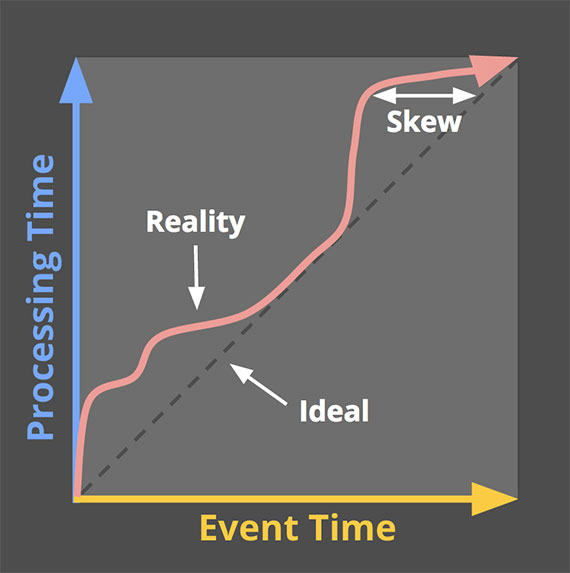
\includegraphics[width=60mm]{img/skew.jpg}
\caption{Adatfolyam feldolgozás a valóságban. \label{skew}}
\end{figure}

\subsection{Lambda architektúra}
A big data megjelenésével, megjelent az igény, hogy ezeket az adatokat közel valós időben tudjuk feldolgozni. Egy fejlettebb megoldásnak tekinthetjük a Lambda architektúrát, ami a kötegelt feldolgozást (batch processing), és a adatfolyam feldolgozást (stream processing) egyesíti. Megalkotása során törekedtek arra, hogy 
\begin{itemize}
\item robosztus, hiba toleráns legyen, mind hardver, mind szoftver oldalon
\item széles körű felhasználhatóság biztosítson, alacsony válaszidővel
\item horizontálisan skálázható legyen (több "általános célű" gép használatával lehessen növelni a teljesítményt)
\item bővíthető legyen
\end{itemize}

Ezen feltételek mellett egy három rétegű architektúrát alkotott meg Nathan Marz~\cite{lambda}. A kötegelési réteg (batch layer), a sebesség réteg (speed layer) és a kiszolgáló réteg (serving layer) biztosítja az adatfeldolgozást. Az adat változatlan formában eljut mind a kötegelt, mind a sebesség rétegbe. A kötegelt réteg tartalmazza a mester adathalmazt, ami nem módosítható, csak egyszer írható formában tárolja az adatokat. Ez a réteg meghatározott időszakonként, ciklikusan lefutattja a számításait, amivel létrehozza az ún. kötegelt nézetet (batch view). Ez a réteg felel azért, hogy az adat pontosan (lehetséges újraszámítás, ahogy érkeznek az újabb adatok) és teljesen jelenjen meg a felhasználó előtt (magas válaszidővel).  A kiszolgáló réteg indexeli ezeket a nézeteket, ezzel biztosítva az ad-hoc, gyors lekérdezéshetőségüket. \linebreak
A sebesség réteg csak friss adatokkal dolgozik, így csökken a pontosság és a teljesség, viszont gyors, inkrementális algoritmusok segítségével, alacsony válaszidővel tudja az adatokat a kimenetre küldeni. A kiszolgáló réteg a kötegelt és a sebesség nézetek összefűzéséből állítja elő az elvárt kimenetet.

\begin{figure}[ht!]
\centering
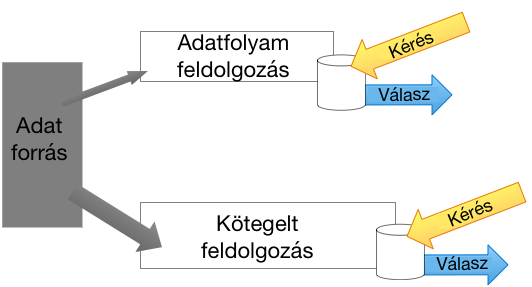
\includegraphics[width=90mm]{img/lambda.png}
\caption{Lambda architektúra felépítése \label{lambda}}
\end{figure}


\subsection{Adatfeldolgozó mintázatok}
Ahhoz, hogy tudjuk mivel dolgozik egy modern, adatfolyam alapú feldolgozó egység, részleteznünk kell az eddig használtakat.

\subsubsection{Kötegelt feldolgozás véges adaton}
Az adatfeldolgozási folyamat nagyon egyszerű, vesszük a különböző típusú adatokat meghatározott időközönként és egy adatfeldolgozó architektúra (pl.: MapReduce~\cite{mapreduce}) segítségével átalakítjuk struktúrált adatokká.

\begin{figure}[ht!]
\centering
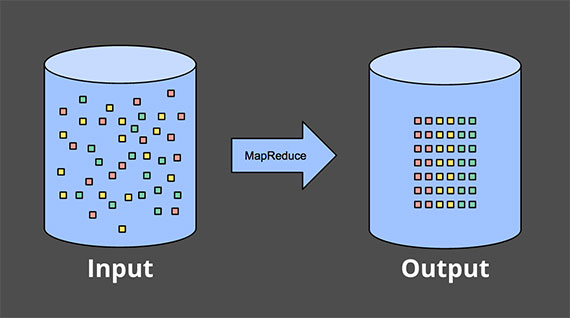
\includegraphics[width=90mm]{img/batch.jpg}
\caption{Bal oldalon található entrópikus adatokból MapReduce segítségével struktúrált, információval rendelkező adatokat generálunk. \label{batchreduce}}
\end{figure}

\subsubsection{Kötegelt feldolgozás végtelen adaton}
\textsl{Végtelen} adatnál még mindig használhatunk kötegelt feldolgozó rendszereket, azzal a kiegészítéssel, hogy az adatok felbontjuk véges részekre, így azok feldolgozhatóvá válnak. Két fő módszertan van elterjed, a rögzített windowing és a session.

\paragraph{Rögzített windowing} arra vonatkozik amely során fix méretű átmenetei időblokkokat vezetünk be, és ezeken az ablakokon futtatjuk le feldolgozó algoritmusunkat. A problémák ennél a megoldásnál nyilvánvalóak. Többidejűséggel (több sorozatban érkezik meg az adat) és többhelyűséggel (több földrajzi elhelyezkedésről érkezik meg az adat) nem tud foglalkozni, így nem tudja biztosítani az adat teljességét és pontosságát.

\paragraph{Sessionnél} valamilyen felhasználói aktivitás alapján meghatározzuk, hogy valószínűleg mennyi ideig fog tartani az adatfolyam. Ez alapján hozok létre ablakokat, melyeken végrehajtom a műveleteimet. Főbb probléma, ha átcsúszik az adat a következő session-be, akkor csak a komplexitás (addícionális logikával) vagy a válaszidő növelésével(növelem a session idejét) tudjuk figyelembe venni.

\subsubsection{Adatfolyam feldolgozás végtelen adaton}
Ebben az esetben az adataink rendezetlenek és nem tudjuk explicit megmondani azt az $epszilon$ időt, ami az adat létrejötte és feldolgozás között van. 4 kategóriába lehet sorolni az ennél a csoportnál alkalmazott technikákat: időfüggetlen (time-agonostic), közelítő algoritmusok, windowing feldolgozási és windowing az adat létrejötte függvényében. 

\paragraph{Időfüggetlen feldolgozás} esetében nem vesszük számításba (és nem is fontos) az, hogy mikor érkeznek meg az adatok, mivel \textsl{adatvezérelt} módon történik a logika meghatározása. Szűrők és inner-join-ok segítségével dolgozunk. Az előbbi esetben mindig csak a soron következő adatról kell eldöntenünk, hogy megfelel-e a feltételeknek (pl.: adott IP címről érkező adatok kategorizálása), míg az utóbbinál egynél több forrásból érkező adatokat úgy kapcsoljuk össze, hogy az elsőnek beérkezett adatot perzisztens módon eltároljuk. 

\paragraph{Becslő algoritmusok} mint például Top-n~\cite{topn} alkotják a második kategóriát az adatfolyam alapú feldolgozó technikáknál. Végtelen adatból egy nagyjából jó, véges kimenetet generálnak, ami egyes esetekben megfelelő adatot eredményez. Ezeknek az algoritmusoknak hátránya, hogy az eredmény nem teljesen jó, illetve általában feldolgozási idő alapján dolgoznak, így a rendezetlen adatoknál pontatlan kimenet lehet az eredmény.

\paragraph{Windowing} létrehozásánál megkülönböztetünk az adat születése és feldolgozása felett működő modellt. A feldolgozás alapú ablakoknál a fő problémánk az, hogy az adataink nem sorrendben érkeznek meg a feldolgozó motorhoz, így előfordulhat, hogy egyes adatok lemaradnak, így rontva a feldolgozás eredményességét. Az adat születése alapú ablaknál viszont tekintettel vagyunk arra, hogy mikor születik az adat, így az azonos időben született adatokat együtt tudjuk feldolgozni.


\section{Gépi tanulás}

Amikor tanulunk, a célünk, hogy minél jobb eredményeket érjünk el a számonkérésen, vagy minél több tudást halmozzunk fel, amit a későbbiek során (valószínűsíthetően) hasznosítani tudunk. A gépi tanulásnak is ugyanez a célja, különböző modellek megalkotása után a megadott példákból (input adat) különböző kimeneteket (output adat) ad ki. Az input adatokból próbál általánosítani oly módon, hogy az felhasználható legyen számára ismeretlen problémák során. Ebből következően minél több bemeneti adatunk és tapasztalatunk (adat) van, annál jobb okosabb és pontosabban fog előrejelezni a használni kívánt algoritmus. Gépi tanulást használunk például: 
\begin{itemize}
\item web keresés
\item spam szűrés
\item ajánló rendszerek
\item online hírdetések
\end{itemize}
esetén is. 
Egy 2011-es Mckinsey riport ~\cite{mckinsey} szerint a gépi tanulás (illetve a prediktív analitika) lesz a következő évek innovációinak alapja. IBM Watson-ja~\cite{watson}, már képes a beadott tünetek alapján, megjósolni, hogy mi lehet a páciens betegsége (egyelőre még csak fejlesztőknek, API-n keresztül). \linebreak

Két fő csoportja van a gépi tanulási algoritmusoknak: a felügyelt (supervised) és nem felügyelt (unsupervised) tanítás.

\subsection{Felügyelt tanítás}

Általánosan fogalmazva, az adat amit betáplálunk a gépi tanulás modellünkbe, tréning példáknak (training set) nevezzük. A tréning példák $x$, $y$ párokat tartalmaznak, ahol $x$ az érték vektor (feature vector). Minden $x$ érték: kategórikus (diszkrét értékeksorozatból származik, pl.: \{kék, piros, sárga\}) vagy numerikus (az érték egész vagy valós szám). $y$ a címke (label), ami kategorizáló érték $x$-re nézve.A célünk az, hogy felfedezzük azt az 
\begin{equation*} y=f(x)
\end{equation*}
függvényt, ahol a legjobban előre tudjuk jelezni az $y$ értéket a meghatározott $x$-re nézve.

Fontos, hogy szétválasszuk az adatainkat tréning és teszt adatokra. Ez biztosítja azt, hogy ne fordulhasson elő az a probléma, hogy a modellünk túlságosan fontos súllyal vesz egyes objektumokat az adatsoron (amik nem jellemzőek a lehetséges valós adatokra), ami azt eredményezi, hogy a valós problémákon már nem fog eredményesen működni. A problémát túltanulásnak vagy magolásnak (overfitting) nevezik. ~\cite{overfit}


\begin{figure}[ht!]
\centering
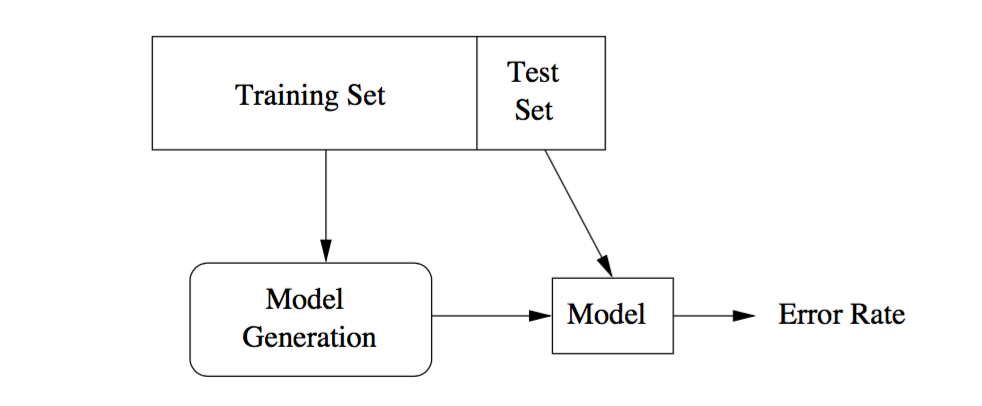
\includegraphics[width=90mm]{img/ml.png}
\caption{Felügyelt tanulás általános modellje \label{ml}}
\end{figure}

\subsection{Nem felügyelt tanítás}
Nem felügyelt tanítás esetén adottak: $(x_1, x_2, ..., x_n)$ adataink, és nincs célfüggvényünk, vagy elvárt kimenetünk. Alapvetően nem struktúrált \textsl{zajból} próbálunk mintázatot keresni, olyan modellt létrehozni, ami jól reprezentálja adatok valószínűségi eloszlálást. Annak ellenére, hogy nincs információnk arról, hogy az egyes adatok milyen kapcsolatban vannak egymással, $(x_t)$ valószínűségi eloszlását meg tudjuk jósolni  $(x_1,x_2, ..., x_{t-1})$ alapján, ahol $P(x_t|x_1,x_2, ..., x_{t-1})$.
Egyszerűbb esetekben, ahol az bemenet sorrend irreleváns, lehet modellt építeni az adatra, ahol $(x_1, x_2, ...)$ az adatsorunk, és ezek függetlenül de egyöntetűen származnak a $P(x)^2$-ból.~\cite{unsupervised}

\section{Ajánlórendszerek}
Az ajánlórendszerek olyan, főként webes rendszerek, ahol a különböző forrásból származó adatok alapján ajánlunk olyan lehetőségeket a felhasználóknak, ami nagy valószínűséggel megfelel a preferenciájának. Például:
\begin{itemize}
\item Youtube, ahol az nézettségi történet alapján kapja az ajánlásokat a felhasználó
\item Amazon, ahol az a cél, hogy a felhasználónak olyan termékeket ajánljunk, amit a hozzá hasonló felhasználók (k-legközelebbi analízis segítségével) is preferálnak. ~\cite{knearest}
\end{itemize}
Két fő fajtáját különböztetjük meg az ajánló rendszereknek. A Content-based (tartalom alapú) ahol az item tulajdonságait vizsgáljuk, illetve a collaborative filtering (együttműködésen alapuló szűrés), ahol a hasonló érdeklődésű felhasználóknak nyújtott ajánlásokat vesszük alapul. \linebreak

Az ajánlórendszerek alapja az ún. rating matrix, ami tartalmazza a felhasználókat és hozzájuk kapcsolt elemek adatait. Minden felhasználó-item párhoz egy értéket rendelünk, ami jellemzi, hogy mennyire preferálja az adott elemet. Ez az érték általában egy rendezett skáláról (pl.: 5 elemű skála, 1-től 5-ig számozva, ahol az 1 a legkevésbé, az 5 pedig a legjobban kedvelt elemet jelöli) kerül ki. Alapfeltevés, hogy a mátrixunk ritka (nincs teljesen kitöltve), mivel nem értékel minden felhasználó minden elemet. A hiányzó, nem ismert értékekről semmilyen explicit információval nem rendelkezünk.

\begin{figure}[ht!]
\centering
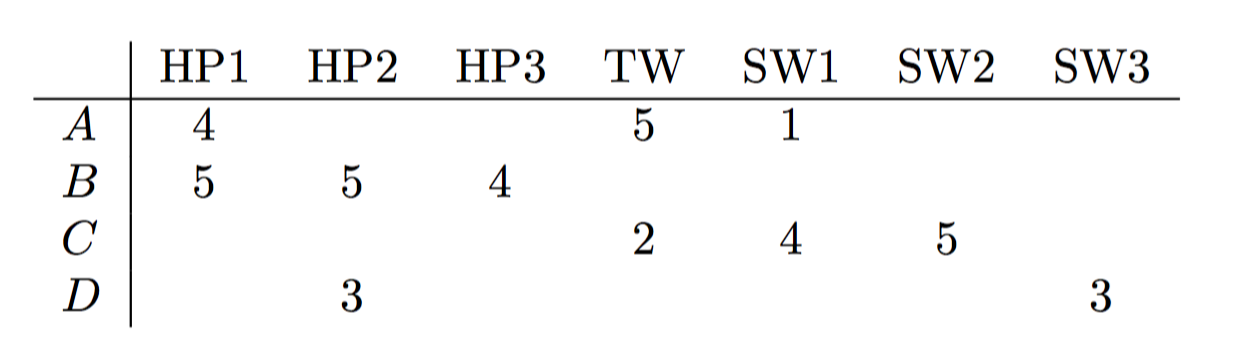
\includegraphics[width=90mm]{img/um.png}
\caption{Rating matrix, ahol az $A,B, C, D$ felhasználók a Star Wars, Harry Potter és Twilight filmeket értékelték \label{um}}
\end{figure}

Célünk az, hogy hiányzó értékeket a mátrixban minél jobban megjósoljuk. Természetesen nem fontos, hogy az összes elemét kitöltsük, törekednünk kell arra, hogy az ajánlás a preferált filmek/cikkek körében legyen, mivel ezek eladása/elolvasása racionalizálható gazdasági szempontból. Jelen esetben, kíváncsiak lehetünk, hogy $A$ felhasználónak ajánlhatjuk-e Harry Potter 2. részét. Láthatjuk, hogy HP 1. részét kedvelte, és tudjuk, hogy a két film kapcsolatban van egymással (rendezők, színészek, történet, stb.) ezért gyaníthatjuk, hogy a második részt is jól fogja értékelni.

\subsection{Hosszú farok}

Amikor bemegyünk egy könyvesboltba, többféle módon is választhatunk egyes könyvek közül. Vannak kiemelt könyvek, amikre nagy az érdeklődés, ezért a könyvesbolt jobban reklámozza ezeket. Személyes ajánlásra nincs lehetőség, a választék korlátozott, erőforrás hiányában az összes könyvnek csak egy szűk szeletét mutatja meg egy könyvesbolt. Ezzel szemben egy online bolt bármit ajánlhat, ami létezhet, nem csak a populárisabbakat, hanem a kevésbé keresetteket is. Ezt a megkülönböztetést nevezzük \textsl{hosszú farok}-nak~\cite{longtail}, és ez az, ami létrehozta az ajánlórendszerek igényét. Muszáj ajánlanunk a felhasználónak termékeket --mivel nincs olyan nyilvánvaló módon prezentálva, mint a fizikai boltoknál-- ahhoz, hogy nagyobb eséllyel vásároljon belőlük.

\subsection{Rating mátrix feltöltése}
Utilty mátrix nélkül nem lehetséges a felhasználóknak ajánlattétel. Ahhoz, hogy feltudjuk tölteni, két általános megközelítés létezik.
\begin{enumerate}
\item Megkérdezzük a felhasználót a véleményéről (pl.: IMDb, ahol a felhasználók a filmeket értékelhetik egy 1-10-es skálán:)~\cite{imdb}: Ebben az esetben a sikerességünk limitált, mivel a felhasználónak nem származik rövid távon gazdasági előnye abból, hogy értékel (természetesen, ha minden film után reális értékelést adna, akkor hosszú távon jobb ajánlásokat kapna). Másrészt az emberi irracionalitás miatt előfordulhat, hogy részrehajlóan (akár pozitív, akár negatív irányban) értékel, ami eltorzíthatja a rating mátrixot. ~\cite{introspection}
\item Megvizsgáljuk a viselkedését: ebben az esetben azt vizsgáljuk, hogy a felhasználó megtekintette/megvette/stb. az adott terméket. Ha igen, explicit 1-el töltjük fel a mátrixot, ha nem akkor 0-val. Tehát, ha megveszünk (vagy csak megnézünk) egy könyvet az Amazonon, akkor 1-el fogja értékelni a rating mátrixban az algoritmus. Így kiküszöbölhetjük azt, hogy a felhasználó, nem szeretne vagy nem tud helyesen értékelni. Hátránya, hogy nehéz súlyozni a különböző véleményeket, mivel csak 1 elemű skálán dolgozunk.
\end{enumerate}

\subsection{ALS}
Mikor ajánlásokat adunk a felhasználónak, a célünk az, hogy a rating mátrixban a hiányzó elemeket megkeressük. Feltételezhetjük, hogy a felhasználó elemei között kapcsolat van (mivel a felhasználó preferenciája vélhetően \textsl{rögzített} egy rövid időszakon belül), ezért különböző optimalizációs eljárásokat alkalmazhatunk. Az egyik legismertebb ilyen eljárás a mátrix faktorizáció (ALS, Alternating Least Squares), ahol az M rating mátrixunkat faktorokra, részmátrixokra bontjuk. \linebreak
Legyen $U$ és $I$ a felhasználók és elemeik sorozata. $U={\{1, ..., U\}}$ és $I={\{1, ..., I\}}$.  Implicit feltöltött rating legyen $M$, ahol a kitöltött elemek 
$r_{ui}$, az üressek (amire szeretnénk ajánlást adni) pedig $\hat{r}_{ui}$. $M$-et felbonthatjuk két részmátrixra, $P$ és $Q$, és inicializáljuk elemeiket megfelelően kis $k$-val. Válasszuk $M$ egy ismert elemét, legyen $X$. Ha ez a választott $X$ eltér a megfelelő $P$ és $Q$ elem szorzatától, akkor változtassuk meg az eltérés irányában. Ha $X$ értéke megegyezik a vizsgált $P$ és $Q$ faktor szorzatával, akkor válasszunk másik $X$-et.

\[
\begin{bmatrix}
    1 & 1 \\
    1 & 1  \\
    1 & 1  \\
    1 & 1  \\
    1 & 1          
\end{bmatrix}
%
\begin{bmatrix}
    1 & 1 & 1 & 1 & 1 \\
    1 & 1 & 1 & 1 & 1        
\end{bmatrix}
=
\begin{bmatrix}
    5 & 4 & ? & ? & 5\\
	? & 4 & ? & ? & ?\\
	5 & ? & ? & ? & 4\\
	5 & 4 & 5 & ? & 5\\
	5 & ? & 4 & ? & 5\\\end{bmatrix}
\]

Ha egyszerre változtatjuk a két részmátrix elemeit, akkor az NP-nehéz probléma, ezért mindig csak az $P$ részmátrixon iterálunk végig amíg $P$ értékei fixálvan vannak. Ha megfelelően jó eredményt kapunk, akkor váltunk a $Q$-ra, ahol megismételjük ezt a műveletet, amíg el nem érjük a konvergencia állapotát. Alapvető probléma még emellett, hogy ha a részmátrixon a változtatás túl kicsi, akkor rengeteg erőforrást elpazarlunk, ha túl nagy, akkor lehet, hogy átugorjuk az optimális megoldást.

\subsection{Gradient descent}

Ahhoz, hogy nagy adatmennyiségben a lehető legkevesebb költséggel (idő, számítási) tudjunk dolgozni, különböző optimalizációs eljárásokat alkalmazunk. A dolgozatomban vizsgált gradient descent egy olyan metódus, aminek a feladata, hogy egy konvex célfüggvény globális minimumát megtalálja. Legyen $J(\theta)$ a célfüggvény, aminek a minimumát keressük, $\alpha$ a tanulási ráta és $j=0, 1, ..., n$ pedig a függvény paraméterei:
\[\theta_j:=\theta_j-\alpha\frac{\delta}{\delta\theta_j}J(\theta)\]~\cite{andrewml}
Veszek egy kezdeti véletlenszerű értéket, ami a függvény paraméter(einek) értéke lesz. Az algoritmus megvizsgálja a paraméterek gradiensét (parciális deriváltját), ami megadja, hogy milyen irányban kell csökkentenem a paramétert ahhoz, hogy a célfüggvényem is csökkenjen. Addig ismétlem a folyamatot, míg konvergenciára nem jutok. Fontos, hogy két ismétlés (update) között az összes paramétert változtatom. \linebreak
Az $\alpha$ tanulási ráta megadja, hogy mekkora lépésközökkel operál az algoritmusom, tehát mekkorát csökkentek (vagy növelek) az adott változóm értékén. Ha túl nagyra veszem, akkor lehet, hogy váltakozva fogok divergálni és konvergálni, míg ha túl kicsire veszem, lehet, hogy csak a lokális minimumot találom meg.

\begin{figure}[ht!]
\centering
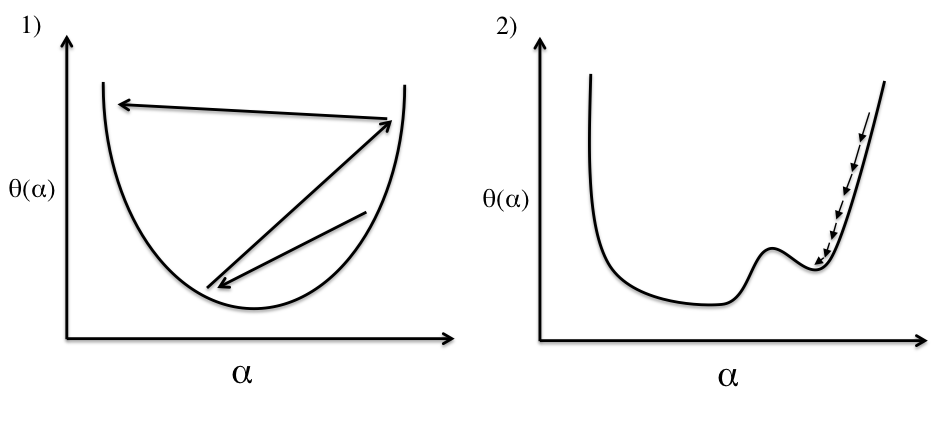
\includegraphics[width=90mm]{img/alfa.png}
\caption{Konvergencia eltévesztése túl nagy és túl kicsi tanulási rátánál \label{alfa}}
\end{figure}

\subsection{Stochastic Gradient descent}


\section{Megvalósítás}

\subsection{Java, Scala}
Dolgozatomban Java és Scala nyelvek alatt fogom implementálni a sztochasztikus gradiens leszállás algoritmust, mivel a Flink is Java alapokon írodott. Java nagyon erős támogatással bír az Apache alapítvány részéről, a 370 támogatott projektből 222 Java alapú. ~\cite{asf} E mellett a rendelkezik olyan tulajdonságokkal, ami a nagyobb, elosztott rendszerek fejlesztésének kezdeténél --'90-es évek közepe és vége-- nagyon kevés nyelv rendelkezett:
\begin{itemize}
\item objektum orientált alapok, mely a nagy komplexitású projektek felépítését megkönnyíti
\item beépített függvénykönyvtár erős hálózati (TCP/IP, UDP, HTTP, stb) támogatással rendelkezik
\item platformfüggetlenség
\item Kivétel és hibakezelés, try/catch
\item hálózati hatás: a Java nyelv elterjedtsége nagyon magas, az egyik legnépszerűbb nyelv a világon ~\cite{tiobe}, ami azt jelenti, hogy nagyon kiterjedt és fejlett külső keretrendszer jellemzi.
\end{itemize}

\paragraph{Scala}--Scalable Language kifejezésből származtatva ~\cite{odersky}-- az elmúlt pár évben lett közismert a nagy adatfeldolgozó, elosztott projektek kapcsán. A vegyes objektum-orientált és funkcionális megközelítés lehetővé teszi, hogy a programozók könnyen átálljanak a nyelvre, mégis kihasználjanak újfajta paradigmákat (first-class functions, immutable data structures, immutability over mutation). Java Virtuális Gép (JVM) alapokon írodott, ezért lehetővé teszi, hogy a megszokott Java könyvtárakkal is dolgozzunk, és emiatt közel azonos sebességre is képes.  E mellett típus-biztos (type-safe), tehát a fordítási időben ellenőrzi a változók típusát és értékét, így elkerülve a futási időben keletkező hibákat~\cite{toptal}. 

\subsection{Flink}
Az Apache alapítvány által támogatott Flink egy olyan valós idejű adatfolyam feldolgolozó architektúra, ami biztosítja, hogy valós időben, végtelen adaton is kellő pontossággal tudjunk műveleteket végezni, anélkül, hogy bonyolult, csak a feladatra tervezett architektúrát kellene létrehoznunk. Ezt az egyszerűséget és pontosságot következő tulajdonságaival éri el ~\cite{flink}
\begin{itemize}
\item egyszerűsített adatfeldolgozó csővezeték (pipeline), amely az adat megkapásától az adat feldolgozásáig tart
\item az adatot olyan módon modellezi és dolgozza fel, ahogy az létrejött, valós-időbeli események alapján
\item nem sorrendben érkezett adatokból származó hibák kiküszöbölése azzal, hogy esemény alapú ablakok létrehozását támogatja
\item biztosítja, hogy a lehető leghamarabb de szükségszerűen legkésőbb történjen az adatfeldolgozás, szem előtt tartva a még meg nem érkezett adatokat
\end{itemize}

\printbibliography

\iffalse
\section{Dcg,nDCG}
\fi

\end{document}
